\section{Results and discussion}\label{results_discussion}
Table \ref{raw_data1} details the performance of the tested ML algorithms on our various datasets. More specifically, Figures \ref{fig:precision} and \ref{fig:auc} respectively compare the precision values and the AUC scores.  
\begin{table}[h]
\resizebox{\textwidth}{!}{
\centering
{
\tiny
{
\begin{tabular}{lcccccc}
\toprule
 \textbf{ML Algorithms} &  \textbf{Datasets} & \textbf{Precision} & \textbf{Recall} & \textbf{F1-score}&\textbf{AUC} &\textbf{Specificity}\tabularnewline
\midrule
 & DT1 &0.97  & 1   & 0.98 & 0.78 & 0.05 \\
& DT2 & 0.59 &0.48 &0.48  &0.64   &0.80\\
& DT3 &0.89  &0.85 &0.87  &0.86   &0.69\\
& DT4 &0.68  &0.57 &0.62  &0.70   &0.74\\
\multirow{-4}{*}{ \textbf{DT}}&   DT5 &0.99  &0.84 &0.91  &0.76   &0.58\\
\midrule
&DT1 &0.97 &1   &0.99 &0.81 & 0.07\\
 & DT2 &0.63  & 0.34  &0.44&0.64& 0.85\\
 & DT3 &0.89 &0.85 &0.87&087&0.70\\
 & DT4 &0.68 &0.56&0.62&0.70&0.74\\
\multirow{-4}{*}{ \textbf{RF}}&   DT5 &0.99 &0.84&0.91&0.76&0.60\\
\midrule
&DT1 &0.97 &1   &0.99 &0.79 &0.05 \\
 &DT2 & 0.58 &0.36   &0.44&0.63&0.81\\
 &DT3 &0.85 &0.88 &0.86&0.86&0.55\\
 &DT4 &0.98 &0.56&0.92&0.70&0.72\\
\multirow{-4}{*}{ \textbf{LR}}&   DT5 & 0.90&0.78&0.88&0.84&0.75\\
\midrule
& DT1 &0.97 &1   &0.99 &0.81 &0.00\\
&DT2 & 0.60 &0.34   &0.43&0.63&0.83 \\
&DT3 &0.86 &0.87 &0.86&0.85&0.60\\
 &DT4 &0.68 &0.59&0.63&0.70&0.73\\
\multirow{-4}{*}{ \textbf{NB}}&0.99 &0.82&0.90&0.84&0.71&0.71\\
\midrule
&DT1 &0.97 &1   &0.99 &0.84 &0.00 \\
&DT2 &0.58  &0.05   & 0.09&0.62&0.97\\
&DT3 &0.57 & 0.86&0.86&0.85&0.64\\
& DT4 & 0.68&0.58&0.62&0.70&0.73\\
 \multirow{-4}{*}{ \textbf{SVM}}& DT5 &0.99 &0.86&0.92&0.80&0.62\\
\midrule
&DT1 &0.97&1 &0.99   &0.84 &0.04  \\
&  DT2 &0.59  &0.40   &0.48&0.65&0.80 \\
& DT3 &0.89 &0.85 &0.87&0.87&0.69\\
& DT4 &0.68 &0.58&0.62&0.70&0.75\\
 \multirow{-4}{*}{ \textbf{ ANN}}&DT5 &0.99 &0.84&0.91&0.79&0.65\\ 
 \bottomrule
\end{tabular}
}
}
}
\caption{All performances measures of our ML models over our five datasets}\label{raw_data1}
\end{table}
%
\begin{figure}[!h]
%\subfigure[Precision values of compared classifiers on different datasets]{
\resizebox{\textwidth}{!}{
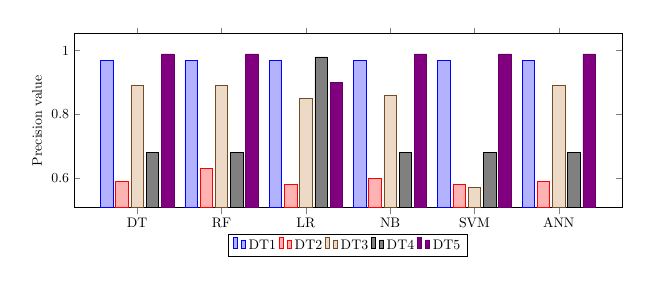
\begin{tikzpicture}[scale=0.5]
 %\centering
\begin{axis}[
     height=6cm, width=15.5cm,
    bar width=0.4cm,
    ybar,
    %ybar=5pt,% configures `bar shift'
    bar width=9pt,
    enlargelimits=0.15,
    legend style={at={(0.5,-0.15)},
    anchor=north,legend columns=-1},
    ylabel={Precision value},
    symbolic x coords={{DT,RF,LR,NB,SVM,ANN}},
    xtick=data,
    %nodes near coords,
    nodes near coords align={vertical},
    ]
\addplot coordinates {(DT,0.97) (RF, 0.97) (LR,0.97)(NB, 0.97)(SVM,0.97)(ANN, 0.97)};
\addplot coordinates{(DT,0.59) (RF, 0.63) (LR,0.58)(NB, 0.60)(SVM,0.58)(ANN, 0.59)};
\addplot coordinates {(DT,0.89) (RF, 0.89) (LR,0.85)(NB, 0.86)(SVM,0.57)(ANN, 0.89)};
\addplot coordinates {(DT,0.68) (RF, 0.68) (LR,0.98)(NB, 0.68)(SVM,0.68)(ANN, 0.68)};
\addplot coordinates {(DT,0.99) (RF, 0.99) (LR,0.90)(NB, 0.99)(SVM,0.99)(ANN, 0.99)};
\legend{DT1,DT2,DT3,DT4,DT5}
\end{axis}
\end{tikzpicture}
}
\caption{Precision values of compared classifiers on different datasets}\label{fig:precision}
\end{figure}
%
\begin{figure}[h]
\resizebox{\textwidth}{!}{
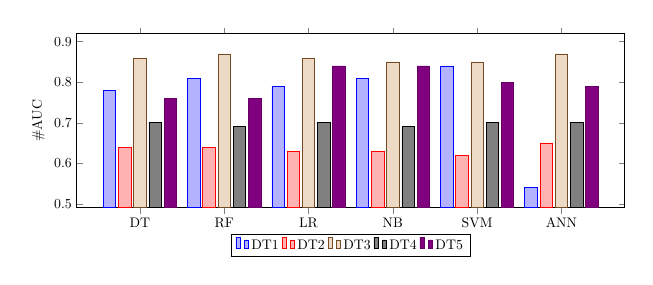
\begin{tikzpicture}[scale=0.5]
 \centering
\begin{axis}[
    height=6cm, width=15.5cm,
    bar width=0.4cm,
    ybar,
    %ybar=5pt,% configures `bar shift'
    bar width=9pt,
    enlargelimits=0.15,
    legend style={at={(0.5,-0.15)},
    anchor=north,legend columns=-1},
    ylabel={\#AUC},
    symbolic x coords={{DT,RF,LR,NB,SVM,ANN}},
    xtick=data,
    %nodes near coords,
    nodes near coords align={vertical},
    ]
\addplot coordinates {(DT,0.78) (RF, 0.81) (LR,0.79)(NB, 0.81)(SVM,0.84)(ANN, 0.54)};
\addplot coordinates{(DT,0.64) (RF, 0.64) (LR,0.63)(NB, 0.63)(SVM,0.62)(ANN, 0.65)};
\addplot coordinates {(DT,0.86) (RF, 0.87) (LR,0.86)(NB, 0.85)(SVM,0.85)(ANN, 0.87)};
\addplot coordinates {(DT,0.70) (RF, 0.69) (LR,0.70)(NB, 0.69)(SVM,0.70)(ANN, 0.70)};
\addplot coordinates {(DT,0.76) (RF, 0.76) (LR,0.84)(NB, 0.84)(SVM,0.80)(ANN, 0.79)};
\legend{DT1,DT2,DT3,DT4,DT5}
\end{axis}
\end{tikzpicture}
}
\caption{Comparison of the AUC values of the ML algorithms on different datasets}\label{fig:auc}
\end{figure}
While an one-all-fits algorithm cannot be deduced from our tests, by closely analyzing the overall performance measures one can observe that RF, LR, SVM, and ANN generally outperform the others for each dataset.  Another important result is that ML algorithms have better precision than RDT 	at least for DT1. 




